\subsection{Graphical notations for probabilistic models}

Probabilistic models can be represented in a diagrammatic format (i.e. a graph or a network) that offers a compact visual representation of complicated systems of probability distributions \cite{Bishop}. In a graphical model the relationship between the nodes becomes more explicit, namely their conditional independence properties which allow the joint distribution over all variables to be factorised into a series of simpler products involving subsets of variables \cite{Bishop}. The basic unit of a network is the node, which represents the different types of variables, including observed variables, unobserved probabilistic variables and unobserved parameters. The nodes are connected by unidirectional edges (arrows) which capture the conditional independence relationship between the variables.

For this thesis we adapted the graphical notations from~\cite{Dietz2010-technical-report-graphs}.

\begin{center}
  \begin{tabular}{m{8cm} m{2cm}}
    Observed variables & \tikz{\node[obs](){$Y$}} \\
    Unobserved probabilistic variables & \tikz{\node[latent](){$\theta$}} \\
    Unobserved parameters & \tikz{\node[latent,double, double distance=1pt](){$\theta$}} \\
    Repetition of node $\theta_n$ for $n\in\llbracket 1;N \rrbracket$ & \tikz{\node[latent](theta){$\theta_n$}; \plate[] {plateN} {(theta)} {$N$};} \\
    Conditional dependency between nodes: $p(Y,\theta) = p(Y|\theta)p(\theta)$ & \tikz{%
            \node[latent]   (theta) {$\theta$};
            \node[obs, xshift=1.5cm] (Y) {$Y$};
            \edge{theta}{Y}}
  \end{tabular}
\end{center}
% For simplicity, fixed hyperparameters are not represented on the graphical model. Unobserved parameters are only represented when optimised together with the unobserved probabilistic variables.

\subsection{Latent variable models for genomics}

With the exponential growth in the use of high-throughput genomics, biological data sets are increasingly high dimensional, both in terms of samples and features. A key principle of biological data sets is that variation between the features results from differences in underlying, often unobserved, processes. Such processes, whether driven by biological or technical effects, are manifested by coordinated changes in multiple features. This key assumption sets off an entire statistical framework of exploiting the redundancy encoded in the data set to learn the (latent) sources of variation in an unsupervised fashion. This is the aim of dimensionality reduction techniques, or latent variable models (LVMs) \cite{Komili2008, Stegle2012, Leek2007, Pournara2007, Dai2017, Genevieve2018, Meng2016}.
%Missing ref Meng2016


\subsubsection{General mathematical formulation}

Given a dataset $\bfY$ of $N$ samples and $D$ features, LVMs attempt to exploit the dependencies between the features by reducing the dimensionality of the data to a potentially small set of $K$ latent variables, also called factors. The mapping between the low-dimensional space and the high-dimensional space is performed via a function $f(\bfX|\bTheta)$ that depends on some parameters $\bTheta$.\\
The choice of $f(\bfX|\bTheta)$ is essentially the field of dimensionality reduction. A trade-off exists between complexity and interpretation: while non-linear functions such as deep neural networks provide more explanatory power, this leads to a considerable challenges in interpretation \cite{Zhang2018_NN}. Hence, for most applications where interpretability is important, $f(\bfX|\bTheta)$ is assumed to be linear \cite{XX}:
% \begin{equation} 
% 	y_{nd} = \sum_{k=1}^{K} w_{dk}z_{n,k}
% \end{equation}
\begin{equation} \label{eq:linear_model}
	\mathbf{Y} = \mathbf{Z}\mathbf{W}^{T}
\end{equation}
where $\bfZ \in \R^{N \times K}$ is a matrix that contains the low-dimensional representation for each sample (i.e. the factors). The matrix $\bfW \in \R^{D \times K}$ contains the weights, which provide the linear mapping between the features and the factors.\\
Note that the aim in dimensionality reduction is to exploit the coordinated heterogeneity between features, and hence features are assumed to be centered without loss of generality.

The inference procedure consists in learning the values of all unobserved variables, including factors and weights. As we shall demonstrate, different inference schemes and assumptions on the prior distributions lead to significantly different model outputs \cite{Rattray2009}.


\subsubsection{Principal component Analysis} \label{section:pca}

Principal Component Analysis (PCA) is the most popular technique for dimensionality reduction \cite{Hotelling1933,Ringner2008}. Starting from \Cref{eq:linear_model}, two formulations of PCA exist \cite{Bishop}. In the maximum variance formulation, the aim is to infer an orthogonal projection of the data onto a low-dimensional space such that variance explained by the projected data is maximised:

\begin{figure}[H]
	\centering
	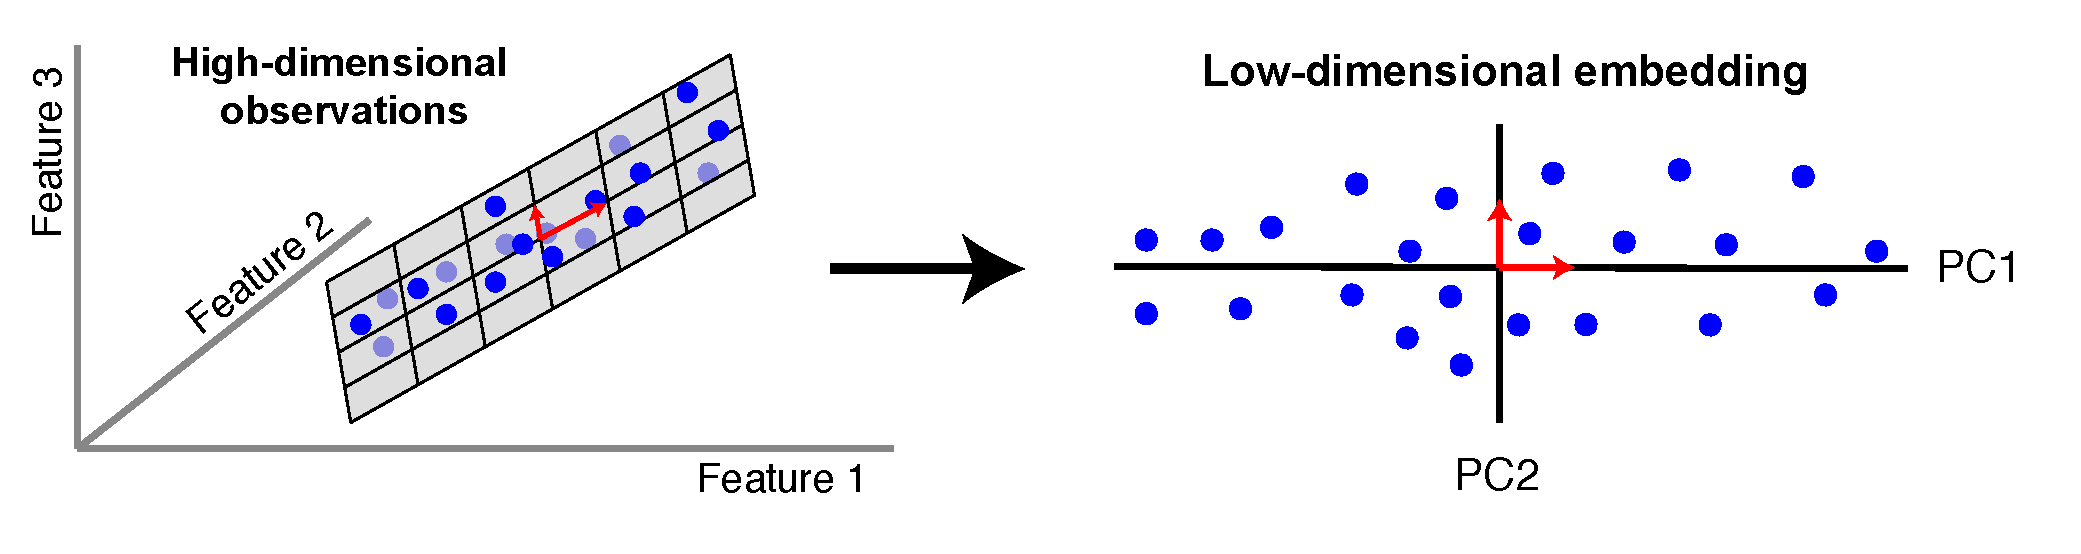
\includegraphics[width=1.0\linewidth]{pca1}
	\caption[]{}
	\label{fig:pca1}
\end{figure}

For a single principal component, the optimisation problem is:
\begin{equation} \label{eq:pca}
	%\argmax_{\|\bfw\|=1} & \sum_{n=1}^{N} (\bfw_1^T \bfy_n)^2 = \\
	\argmax_{\|\bfw\|=1} = \bfw_1^T \bfY^T \bfY \bfw
\end{equation}

where $\bfY^T \bfY=\bfS \in \R^{D \times D}$ is the data covariance matrix and $\bfw_1^T$ is the vector of weights. \\
The $k$-th principal component can be found by subtracting from $\bfY$ the reconstructed data by the previous $k-1$ principal components. If we define $\bfz_k=\bfw_k^T \bfY$ to be the $k$-th principal component:
\[
	\hat{\bfY} = \bfY - \sum_{k=1}^{K} (\bfz_k \bfw_k^T)
\]
Re-applying \Cref{eq:pca} defines the new optimisation problem.

In its minimum error formulation, the aim is to find an equivalent projection that minimises the mean squared error between the observations and the data reconstructed using all principal components:
\[
	\argmax_{\|\bfw\|=1} \Vert \bfY - \sum_{k=1}^{K} (\bfz_k \bfw_k^T) \Vert^{2}
\]
where $\Vert \cdot \Vert^{2}$ is the Frobenius norm.

In both cases, solving the optimisation problems via Lagrange multipliers leads, remarkably, to the same solution:
\begin{equation}
	\bfS \bfw_k = \lambda_k \bfw_k
\end{equation}
Hence, the loading vectors $\bfw_k$ are the eigenvectors of $\bfS$, which can be computed via singular value decomposition \cite{Bishop}.

The reason why the maximum variance solution and the minimum reconstruction error solution are the same can be understood by applying Pythagoras theorem to the right triangle defined by the projection of a sample $\bfy_{n}$ to a loading vector $\bfw$ (\Cref{fig:pca2}).
Assuming again centered data, the variance of $\bfy_{n}$ is $\|\bfy_{n}\| = \bfy_{n}^T \bfy_{n}$. This variance decomposes as the sum of the variance in the latent space $\|\bfz_{n}\| = \bfz_{n}^T \bfz_{n}$ and the residual variance after reconstruction $\|\bfy_{n} - \bfz_{n} \bfw^T \|$:

\begin{figure}[H]
	\centering
	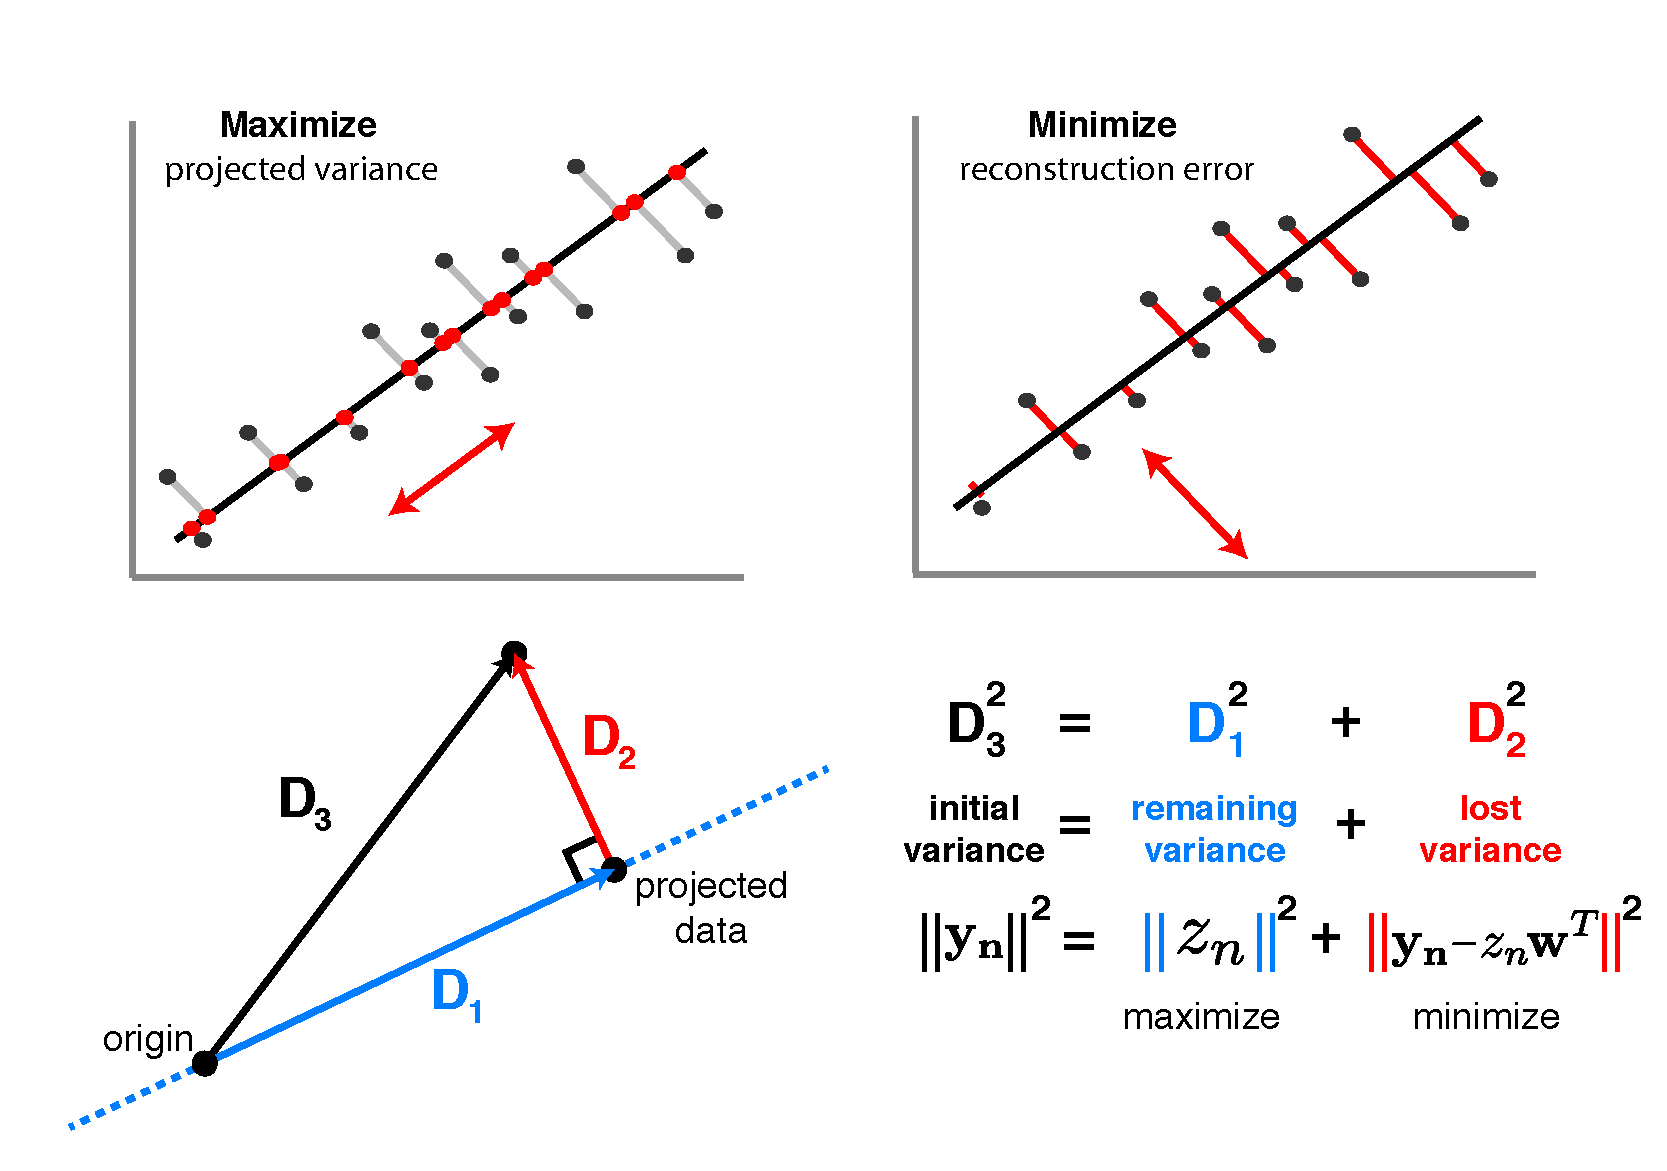
\includegraphics[width=0.9\linewidth]{pca2}
	\caption[Maximizing the variance in the principal component space is equivalent to minimizing the data reconstruction error]{In the maximum variance formulation we aim at maximising the variance of the projected data (blue line), whereas in the minimum error formulation we are aimed at minimising the residual variance (red line). Given a fixed total variance (black line), both strategies are equivalent}
	\label{fig:pca2}
\end{figure}

The main strength of PCA relies on its simplicity and closed form solution. Additionally, the linear mapping has the advantage of yielding interpretable feature weights, so that inspection of $\bfw_k$ reveals which features are jointly affected by the $k$-th principal component.\\
However, PCA suffers from serious drawbacks when applying it to real data sets \cite{Li2017b}. First, biological measurements are inherently noisy, and there is no explicit account of noise in PCA. In practice, high variance components are often asociated with signal whereas low-variance components are assumed to be noise, but an ideal model should explicitly disentangle the uncoordinated variability that is attributed to noise from the coordinated variability that is characterised as signal. Second, in its original formulation, no missing data is allowed \cite{Ilin2010}. Third, there is no rationality on how to evaluate the fit and perform model selection. Finally, it does not offer a principled way of modelling prior information about the data.

\subsubsection{Probabilistic Principal Component Analysis and Factor Analysis} \label{section:probabilistic_pca}
A probabilistic version of PCA was initially proposed in \cite{Tipping1999}. It can be formulated by converting some (or all) fixed parameters into random variables and adding an explicit noise term to \Cref{eq:linear_model}:
\begin{equation}
	\bfY = \bfW \bfZ + \bepsilon
\end{equation}
where the weights $\bfW$ are assumed to be non-probabilistic parameters, but the noise $\bepsilon$ and the latent variables $\bfZ$ (the principal components) are assumed to follow an isotropic normal distribution:
\begin{align*}
	p(\bfZ) &= \prod_{n=1}^{N} \prod_{k=1}^{K} \Ndist{z_{nk}}{0,1} \\
	p(\epsilon) &= \Ndist {\epsilon}{0,\sigma^2}
\end{align*}
%The alternative strategy of treating $\bfZ$ as random variables and $\bfW$ as parameters has also been explored \cite{Lawrence2005}.\\

All together, this leads to a normally-distributed likelihood:
\begin{equation} \label{eq:ppca_lik}
	% p(\bfY|\bfW,\bfZ,\sigma) = \Ndist{\bfY}{\bfW \bfZ,\sigma^2 \I}
	p(\bfY|\bfW,\bfZ,\sigma) = \prod_{n=1}^{N} \prod_{d=1}^{D} \Ndist{y_{n,d}}{\bfw_{,:k}^T \bfz_{n,:},\sigma^2 \I}
\end{equation}

The corresponding graphical model is:

\begin{figure}[H]
	\centering
	% \definecolor{colD}{rgb}{0.2, 0.2, 0.6}
\definecolor{colM}{rgb}{0.0, 0.5, 0.0}
\definecolor{colN}{rgb}{0.5, 0.0, 0.13}
\definecolor{colG}{rgb}{1.0, 0.65, 0.0}
\newcommand\op{0.25}
\colorlet{shadecolor}{black!25}


\begin{tikzpicture}

% Define nodes
\node[obs]   (Y) {$y_{n,d}$};
\node[latent, xshift=-1.5cm, above=of Y, yshift=-0.4cm] (Z) {$z_{n,k}$};
\node[latent, double, double distance=1pt, above=of Y, yshift=0.6cm] (W) {$w_{d,k}$};
\node[latent, double, double distance=1pt, xshift=1.5cm] (Tau) {$\tau$};

% Connect the nodes
\edge {Z,W, Tau} {Y};

% Plates
\plate[] {plateK} {(Z)(W)} {$K$};
\plate[] {plateN} {(Y)(Z)(plateK.south east)(plateK.south west)} {$N$};
\plate[] {plateD} {(Y)(W)(plateK.north east)(plateN.south east)} {$D$};

\end{tikzpicture}
	\caption{Graphical model for probabilistic PCA. The latent variables are modelled as random variables, whereas the weights and the noise are modelled as deterministic parameters.}
	\label{fig:pPCA}
\end{figure}

Importantly, the choice of the distribution for $\epsilon$ implies that the noise of each feature is independent but restricted to have the same variance $\sigma$. In practice this is a limiting assumption, as different features are expected to show different degrees of noise, albeit this constraint can be relaxed and forms the basis of Factor Analysis \cite{Rubin1982,Bishop}.

The inference procedures involves learning the parameters $\bfW$, and $\sigma^2$ and a posterior probability distribution for $\bfZ$. As the model depends on latent variables, inference can be performed using the iterative Expectation-Maximisation (EM) algorithm \cite{Rubin1982,Bishop}. In the expectation step, the posterior distribution for $\bfZ$ is computed in closed form (due to conjugacy between the likelihood and the prior), given current estimates for the parameters $\bfW$, and $\sigma^2$. In the maximisation step, the parameters are calculated by maximising the expectation of the joint log likelihood under the posterior distribution of $\bfZ$ found in the E step \cite{Tipping1999}.\\
Interestingly, the EM solution of probabilistic PCA lies in the same subspace than the traditional PCA solution \cite{Tipping1999}, but the use of a probabilistic framework brings several benefits. First, model selection can be performed by comparing likelihoods across different settings of parameters. Second, missing data can naturally be accounted for by ignoring the missing observations from the likelihood. Finally, the probabilistic formulation sets the core framework for a Bayesian treatment of PCA, enabling a broad range of principled extensions tailored different types of data sets.


\subsubsection{Bayesian Principal Component Analysis and Bayesian Factor Analysis} \label{section:bayesian_pca}

The full Bayesian treatment of PCA requires the specification of prior probability distributions for all unobserved variables:
\begin{align*}
	p(\bfZ) &= \prod_{n=1}^{N} \prod_{k=1}^{K} \Ndist{z_{nk}}{0,1} \\
	p(\bfW) &= \prod_{d=1}^{D} \prod_{k=1}^{K} \Ndist{w_{dk}}{0,1} \\
	p(\epsilon) &= \Ndist {\epsilon}{0,\tau^{-1}} \\
	p(\tau) &= \Gdist{\tau}{a_0,b_0}
\end{align*}
where $\tau$ is the precision (inverse of the variance) of the noise term. A generalisation to Bayesian Factor Analysis follows by allowing a separate noise term per feature:
\begin{align*}
	p(\bepsilon) &= \prod_{d=1}^{D} \Ndist {\epsilon_d}{0,\tau_d^{-1}} \\
	p(\btau) &= \prod_{d=1}^{D} \Gdist{\tau_d}{a_0,b_0}
\end{align*}
where $a_0$ and $b_0$ are fixed hyperparameters. As in \Cref{eq:ppca_lik}, this results in a Normal likelihood:
\[
	p(\bfY|\bfW,\bfZ,\btau) = \prod_{n=1}^{N} \prod_{d=1}^{D} \Ndist{y_{nd}}{\bfw_{d}^T \bfz_{n},\tau_d}
\]

The corresponding graphical model is:

\begin{figure}[H] 
	\centering
	\begin{tikzpicture}

% Define nodes
\node[obs]   (Y) {$y_{n,d}$};
\node[latent, above=of Y, xshift=-1.5cm] (Z) {$z_{n,k}$};
\node[latent, above=of Y, xshift=1.5cm] (W) {$w_{d,k}$};
\node[latent, xshift=1.5cm] (Tau) {$\tau_{d}$};

% Connect the nodes
\edge {Z,W, Tau} {Y};

% Plates
\plate[] {plateK} {(Z)(W)} {$K$};
\plate[] {plateN} {(Y)(Z)(plateK.north west)} {$N$};
\plate[] {plateD} {(Y)(W)(Tau)(plateK.south east) (plateN.south east) (plateN.north east)} {$D$};

\end{tikzpicture}
	\caption{Graphical model for Bayesian Factor Analysis. All unobserved variables are modelled as random variables.}
	\label{fig:bayesianFA}
\end{figure}

\subsubsection{Hierarchical priors: Automatic relevance determination} \label{section_ard}

A key advantage of the full Bayesian treatment is that it explicitly captures uncertainity on the estimation of all unobserved variables, as opposed to the probabilistic PCA model \cite{Bishop1999a,Bishop1999b}. Yet, more importantly, the use of (hierarchical) prior distributions allow different modelling assumptions to be encoded, providing a flexible and principled approach to extend PCA to a myriad of modelling scenarios, including multi-view generalisations \cite{Klami2008,Virtanen2012,Klami2015,Bunte2016,Khan2014,Zhao2016}.

As an example, a major challenge in PCA is how to determine the dimensionality of the latent space (i.e. the number of principle components). As we will show, the use of hierarchical prior distributions allows the model to introduce sparsity assumptions on the weights in such a way that the model automatically learns the number of factors.\\
In the context of Factor Analysis, one the first sparsity priors to be proposed was the Automatic Relevance determination (ARD) prior \cite{Neal1995,Mackay1996,Bishop1999a,Bishop1999b}. 
\begin{equation*} \label{eq:ard}
	p(\bfW|\balpha) = \prod_{k=1}^{K} \Ndist{\bfw_{:,k}}{0,\frac{1}{\alpha_{k}}\I_{D}} \\
	\qquad\qquad
	p(\balpha) = \prod_{k=1}^{K} \Gdist{\alpha_k}{a_0^\alpha, b_0^\alpha}
\end{equation*}
The aim of this prior is two-fold. First, the zero-mean normal distribution specifies that, \textit{a priori}, no information is available and all features are \textit{inactive}. When exposed to some data, the posterior distribution for $\bfW$ will be estimated by weighting the contribution from the likelihood, potentially allowing features to escape from the zero-centered prior (\Cref{fig:ard}).\\
Second, performing inference on the variable $\balpha = \{ \alpha_1, \cdots, \alpha_k \}$ enables the model to discard inactive factors. To understand this, let us assume that only $K=5$ true factors exist, but the model is initialised with $K=20$ factors. In such case, inactive factors can be prunned out by driving the corresponding $\alpha_k$ to infinity. In turn, this causes the posterior $p(\bfw_{:,k}|\bfY)$ to be sharply peaked at zero, resulting in the inactivation of all its weights \Cref{fig:hinton}.

\begin{figure}[H] \begin{center}
	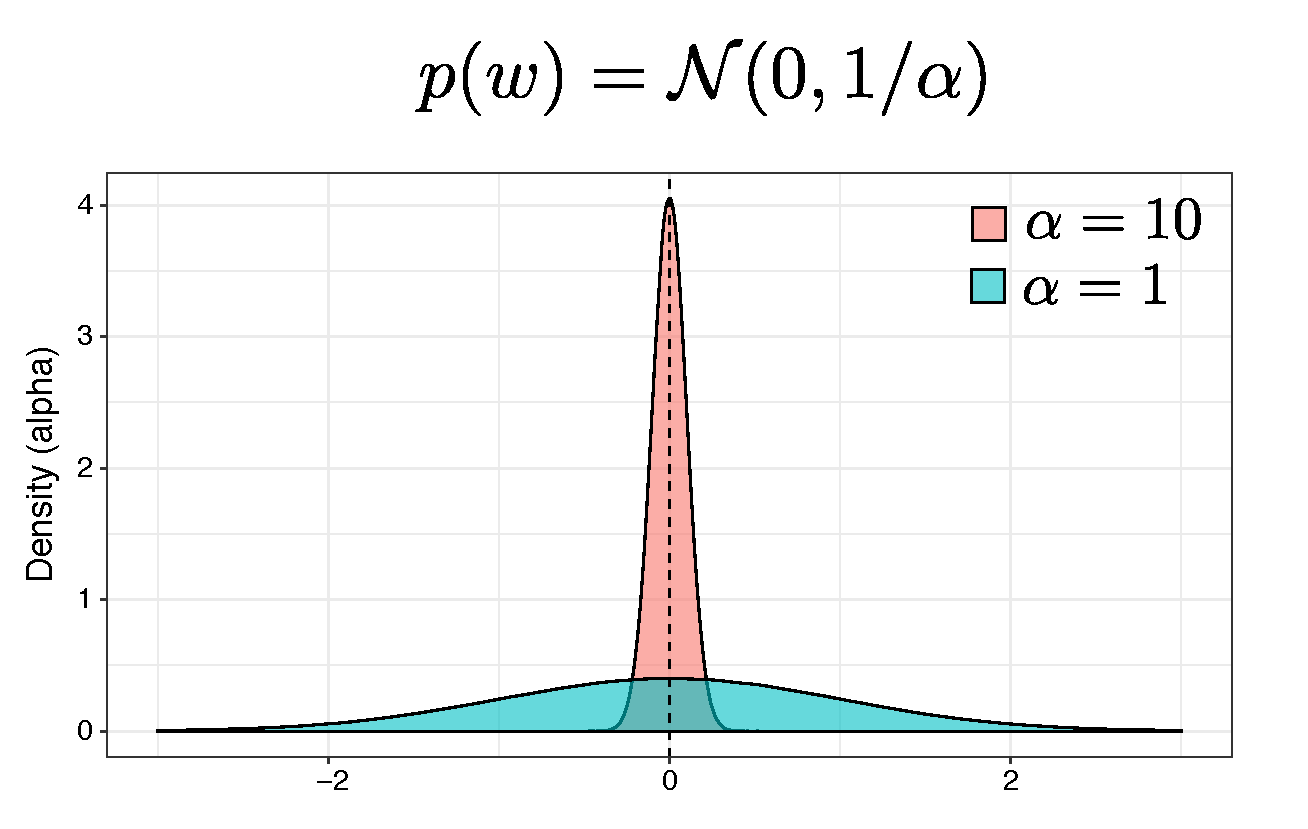
\includegraphics[width=0.7\textwidth]{Chapter2/Figs/ard}
	\caption{Visualisation of the sparsity-inducing Automatic Relevance Determination prior}
	\label{fig:ard}
\end{center} \end{figure}

\begin{figure}[H] \begin{center}
	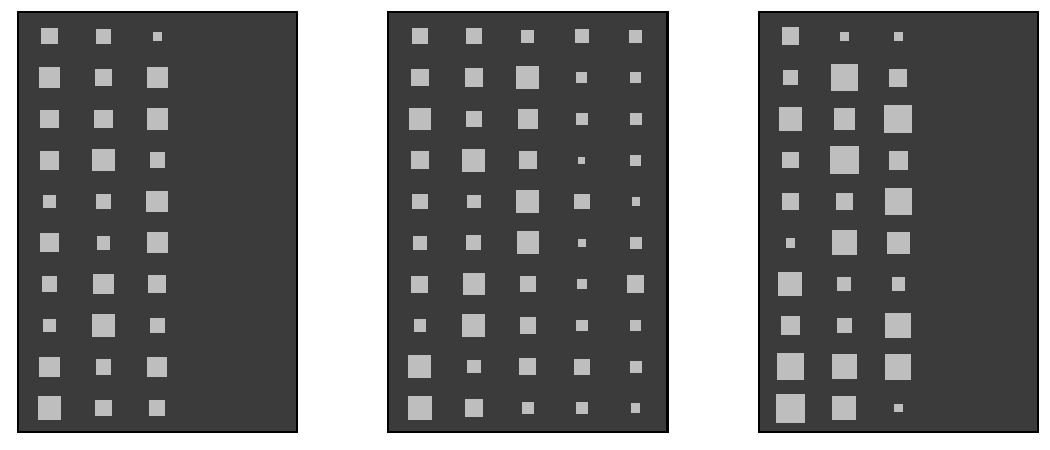
\includegraphics[width=0.8\textwidth]{Chapter2/Figs/hinton}
            \caption[(Copied from Damien's thesis) Hinton plot of the loading matrix for a Bayesian Factor Analysis model with an ARD prior]{Hinton plots display the values of the loading matrix, similar to a heatmap, where bigger squares depict larger weights. Shown are the Hinton plots for (a) the true weights, (b) the infered weights by a Factor Analysis model with no ARD prior (middle), and (c) the infered weights by a Factor Analysis model with ARD prior per factor. This figure was generated using simulated data with $N=100$ samples, $D=10$ features and $K=3$ factors.}
	\label{fig:hinton}
\end{center} \end{figure}

\subsubsection{Hierarchical priors: Spike-and-slab prior} \label{section_spikeslab}

Sparse extensions of the Bayesian factor analysis model have been proposed as a regularisation mechanism but also to model inherent assumptions regarding the sparse nature of biological data \cite{Stegle2012,Gao2013}.\\
The variability observed in biological data is driven both by technical factors and biological factors. Thechnical factors (i.e. batch effects) tend to be relatively strong and alter the expression of a large proportion of genes, whereas the biological factors are potentially weak effects driven by changes in small gene regulatory networks \cite{Gao2013}. Hence, a practical factor analysis model should be able to learn factors with different degrees of sparsity.\\
The ARD prior proposed in \Cref{eq:ard} allows entire factors to be dropped out from the model, but it provides a weak degree of regularisation when it comes to inactivating individual weights within the active factors.

A sparse generalisation of the Factor Analysis model proposed above can be achieved by combining the ARD prior with a spike-and-slab prior \cite{Mitchell1988,Titsias2011}:
\begin{align}
	p(w_{d,k} \mid \alpha_k,\theta_k) &= (1-\theta_k) \mathds{1}_0(w_{d,k}) + \theta_k \Ndist{w_{d,k}}{0, \alpha_k^{-1}} \\
	p(\theta_k) &= \Bdist{\theta_k}{a_0^\theta,b_0^\theta} \\
	p(\alpha_k) &= \Gdist{\alpha_k}{a_0^\alpha, b_0^\alpha}
\end{align}

The corresponding graphical model is:

\begin{figure}[H] \begin{center}
	\begin{tikzpicture}

% Define nodes
\node[obs]   (Y) {$y_{n,d}$};
\node[latent, above=of Y, xshift=-1.5cm] (Z) {$z_{n,k}$};
\node[latent, above=of W, xshift=-0.75cm] (Theta) {$\theta_{k}$};
\node[latent, above=of W, xshift=0.75cm] (Alpha) {$\alpha_{k}$};
\node[latent, above=of Y, xshift=1.5cm] (W) {$w_{d,k}$};
\node[latent, xshift=1.5cm] (Tau) {$\tau_{d}$};

% Connect the nodes
\edge {Theta, Alpha} {W};
\edge {Z, W, Tau} {Y};

% Plates
\plate[] {plateK} {(Z)(W)(Theta)(Alpha)} {$K$};
% \plate[] {plateN} {(Y)(Z)(plateK.north west)} {$N$};
\plate[] {plateN} {(Y)(Z)} {$N$};
\plate[] {plateD} {(Y)(W)(Tau)(plateK.south east) (plateN.south east) (plateN.north east)} {$D$};

\end{tikzpicture}
	\label{fig:bayesianFA}
	\caption{Graphical model for Bayesian sparse Factor Analysis. A double sparsity-inducing prior is used on the weights: an ARD prior to prune inactive factors and a spike-and-slab prior to inactive individual features within the active factors.}
\end{center} \end{figure}

The spike-and-slab prior is effectively a mixture model where features are sampled from a zero-inflated Gaussian distribution, where $\theta_k \in (0,1)$ dictates the level of sparsity per factor (i.e. how many active features). A value of $\theta_k$ close to $0$ implies that most of the weights of factor $k$ are shrinked to $0$ (i.e. a sparse factor), whereas a value of $\theta_k$ close to $1$ implies that most of the weights are non-zero (i.e. dense factors). By learning $\theta_k$ from the data, the model naturally accounts for combinations of sparse and dense factors.


% \subsubsection{Inference}
% In a fully Bayesian setting, the inference procedure corresponds to learning the posterior distributions for each unobserved variable. However, applying Bayes rule yields an analytically intractable solution, and approximate methods are required. This is discussed in Chapter X.



\subsection{Multi-view factor analysis models}

Probabilistic PCA and Factor Analysis perform dimensionality reduction from a single input matrix. In some occasions data is collected from multiple data sources that exibit heterogeneous statistical properties, resulting in a structured data set where features are naturally partitioned into views \cite{Xu2013,Li2016,Zeng2018}. A clear biological example is multi-omics data, where, for the same set of samples, multiple molecular layers are profiled. Each of the data modalities can be analysed separately using conventional (single-view) methods, but in the ideal strategy a single model should be used to leverage information across all molecular layers using a flexible and principled approach. This is refered to as the multi-view learning problem \cite{Xu2013,Li2016}.\\
A tempting approach to circumvent the multi-view learning problem is to simply concatenate all different data sets before applying conventional (single-view) latent variable models \cite{Ritchie2015}. However, this is prone to fail for several reasons. First, heterogeneous data modalities cannot always be modelled using the same likelihood function. For example, continuous measurements are often modelled using a normal distribution, but binary and count-based traits are not appropriately modelled by this distribution \cite{Pilling2018}. Second, even if all views are modelled with the same likelihood, differences in the scale and the magnitude of the variance can lead to some views being overrepresented in the latent space. Finally, in a multi-view data set we expect multiple sources of variation, some of which driven by a single view, whereas others could capture shared variability across multiple views. In other words, from a structured input space, one can also expect a structured latent representation. Not taking this behaviour into account can lead to challenges in the interpretability of the latent space.

A comprehensive review of multi-view machine learning methods can be found in \cite{Xu2013} and a more genomics-oriented perspective can be found in \cite{Ritchie2015}. For the purpose of this thesis, we will describe only the use of latent variable models for multi-view data integration.

\subsubsection{Canonical Correlation Analysis} \label{cca}
Canonical Correlation Analysis (CCA) is a simple extension of PCA to find linear components that capture correlations between two datasets \cite{Hotteling1936,Hardle2007}.\\
Given two data matrices $\bfY_1 \in \R^{N \times D_1}$ and $\bfY_2 \in \R^{N \times D_2}$ CCA finds a set of linear combinations $\bfU \in \R^{D_1 \times K}$ and $\bfV \in \R^{D_2 \times K}$ with maximal cross-correlation.
For the first pair of canonical variables, the optimisation problem is:
\[
	(\hat{\bfu_1}, \hat{\bfv_1}) = \argmax_{\bfu_1,\bfv_1} corr(\bfu_{1}^T \bfY_1, \bfv_{1}^T \bfY_2)
\]
As in conventional PCA, the linear components are constraint to be orthogonal. Hence, the first pair of canonical variables $\bfu_1$ and $\bfv_1$ contain the linear combination of variables that have maximal correlation. Subsequently, Therefore, the second pair of canonical variables $\bfu_2$ and $\bfv_2$ is found out of the residuals of the first canonical variables.

Given the similarity with PCA, both methods share statistical properties, including the linear mapping between the low-dimensional space and the high-dimensional space, and the closed-form solution using singular value decomposition \cite{Hotteling1936,Hardle2007}.\\
Because of its simplicity and efficient computation, CCA has widespread use as a dimensionality reduction technique \cite{Hardle2007}. Yet, as expected, CCA suffers from the same pitfalls as PCA: difficulties in selecting the number of components, lack of sparsity in the solutions and absence of probabilistic formulation. In addition, CCA have been shown to overfit for datasets where $D>>N$ \cite{McCabe2018,Guo2016}. Hence, probabilistic versions with sparsity assumptions that reduce overfitting and improve interpretability followed.


\subsubsection{Probabilistic Canonical Correlation Analysis} \label{section_probabilisticCCA}

Following the derivation of probabilistic PCA \cite{Tipping1999}, a similar effort enabled a probabilistic formulation of CCA as a generative model \cite{Bach2005}.\\
In this model, the two matrix of observations $\bfY^{1}$ and $\bfY^{2}$ are decomposed in terms of two loading matrices $\bfW^{1}$ and $\bfW^{2}$ but a joint latent matrix $\bfZ$:
\begin{align*}
	\bfY^{1} &= \bfW^{2} \bfZ + \epsilon^{1} \\
	\bfY^{2} &= \bfW^{2} \bfZ + \epsilon^{2}
\end{align*}
With the following prior probability distributions:
\begin{align*}
	p(z_{nk}) &= \Ndist{z_{nk}}{0,1} \\
	p(\epsilon^{1}) &= \Ndist {\epsilon^{1}}{\tau_{1}^{-1}} \\
	p(\epsilon^{2}) &= \Ndist {\epsilon^{2}}{\tau_{2}^{-1}}
\end{align*}
As in \cite{Tipping1999}, the weights and the variance of the noise are assumed to be non-probabilistic parameters, whereas the factors are probabilistic unobserved variables. This yields the following likelihood functions:
\begin{align} \label{eq:probabilistic_cca_likelihood}
	p(\bfY^{1}|\bfW^{1},\bfZ,\tau_{1}) &= \prod_{n=1}^{N} \prod_{d=1}^{D_1} \Ndist{y^{1}_{n,d}}{(\bfw_{:,k}^{1})^T \bfz_{n},\tau_{1}^{-1}} \\
	p(\bfY^{2}|\bfW^{2},\bfZ,\tau_{2}) &= \prod_{n=1}^{N} \prod_{d=1}^{D_2} \Ndist{y^{2}_{n,d}}{(\bfw_{:,k}^{2})^T \bfz_{n},\tau_{2}^{-1}} \nonumber
\end{align}

The corresponding graphical model is:

\begin{figure}[H] \begin{center}
	\begin{tikzpicture}

% Define nodes
\node[obs, xshift=-1.5cm] (Y1) {$y^{1}_{n,d}$};
\node[obs, xshift=+1.5cm] (Y2) {$y^{2}_{n,d}$};

\node[latent, below=of Y1, yshift=+0.5cm, xshift=+1.5cm] (Z) {$z_{n,k}$};

\node[latent, double, double distance=1pt, below=of Y1, xshift=-1cm, yshift=-1cm] (W1) {$w^{1}_{d,k}$};
\node[latent, double, double distance=1pt, below=of Y2, xshift=+1cm, yshift=-1cm] (W2) {$w^{2}_{d,k}$};

\node[latent, double, double distance=1pt, left=of Y1, yshift=-0.5cm] (Tau1) {$\tau^{1}$};
\node[latent, double, double distance=1pt, right=of Y2, yshift=-0.5cm] (Tau2) {$\tau^{2}$};

% Connect the nodes
\edge {Z} {Y1};
\edge {Z} {Y2};
\edge {W1} {Y1};
\edge {W2} {Y2};
\edge {Tau1} {Y1};
\edge {Tau2} {Y2};
% \edge {Z,W, Tau} {Y};

% Plates
\plate[] {plateK} {(Z)(W1)(W2)} {$K$};
% \plate[] {plateN} {(Y1)(Y2)(Z)(plateD1.north)} {$N$};
% \plate[] {plateD1} {(Y1)(W1)(plateK.south)(plateN.north)} {$D_1$};
% \plate[] {plateD2} {(Y2)(W2)(plateK.south)(plateN.north)} {$D_2$};
\plate[] {plateN} {(Y1)(Y2)(Z)} {$N$};
\plate[] {plateD1} {(Y1)(W1)(Tau1)} {$D_1$};
\plate[] {plateD2} {(Y2)(W2)(Tau2)} {$D_2$};

\end{tikzpicture}



	\label{fig:graphical_CCA}
	\caption{Graphical model for probabilistic Canonical Correlation Analysis}
\end{center} \end{figure}

Notice that the observations for both data sets are generated from the same set of latent variables $\bfZ$. This ensures that the model is focused on capturing the variation associated with cross-correlated groups of features.\\
Analogously to probabilistic PCA, the expected value of the posterior distribution $p(\bfZ|\bfY^{1},\bfY^{2})$ span the same subspace as standard CCA \cite{Bach2005}. Nonetheless, one of the many advantage of a probabilistic formulation is that it enables a broad range of principled extensions into larger graphical models.


\subsubsection{Bayesian Canonical Correlation Analysis} \label{section:bayesian_cca}
A fully Bayesian treatment of CCA followed based on exactly the same principle presented in \Cref{section:bayesian_pca} by introducing prior distributions to all unobserved variables \cite{Wang2007,Klami2013}:
\begin{align*} 
	p(\bfZ) &= \prod_{n=1}^{N} \prod_{k=1}^{K} \Ndist{z_{nk}}{0,1} \\
	p(\epsilon^{1}) &= \Ndist {\epsilon^{1}}{\sigma_{1}^{2}} \\
	p(\epsilon^{2}) &= \Ndist {\epsilon^{2}}{\sigma_{2}^{2}} \\
	p(\bfW^1|\balpha) &= \prod_{k=1}^{K} \Ndist{\bfw^{1}_{:,k}}{0,\frac{1}{\alpha_{k}}\I_{D_1}} \\
	p(\bfW^2|\balpha) &= \prod_{k=1}^{K} \Ndist{\bfw^{2}_{:,k}}{0,\frac{1}{\alpha_{k}}\I_{D_2}} \\
	p(\balpha) &= \prod_{k=1}^{K} \Gdist{\alpha_k}{a_0^\alpha, b_0^\alpha}
\end{align*}
Resulting in the same likelihood model as in \Cref{eq:probabilistic_cca_likelihood}. Yet, notice that an ARD is introduced per factor, allowing an automatic inference of the dimensionality in the latent subspace.
Also, there is some flexibility in the definition of noise. An independent noise term can be defined per view or per per feature. One could also model correlated noise by generalising the distribution to a multivariate Gaussian with full-rank covariance. \cite{Wang2007,Klami2013}.

The corresponding graphical model is:

\begin{figure}[H] \begin{center}
	\begin{tikzpicture}

% Define nodes
\node[obs, xshift=-1.5cm] (Y1) {$y^{1}_{n,d}$};
\node[obs, xshift=+1.5cm] (Y2) {$y^{2}_{n,d}$};

\node[latent, below=of Y1, yshift=+0.5cm, xshift=+1.5cm] (Z) {$z_{n,k}$};

\node[latent, below=of Y1, xshift=-1cm, yshift=-1cm] (W1) {$w^{1}_{d,k}$};
\node[latent, below=of Y2, xshift=+1cm, yshift=-1cm] (W2) {$w^{2}_{d,k}$};

\node[latent, left=of Y1, yshift=-0.5cm] (Tau1) {$\tau^{1}$};
\node[latent, right=of Y2, yshift=-0.5cm] (Tau2) {$\tau^{2}$};

% Connect the nodes
\edge {Z} {Y1};
\edge {Z} {Y2};
\edge {W1} {Y1};
\edge {W2} {Y2};
\edge {Tau1} {Y1};
\edge {Tau2} {Y2};
% \edge {Z,W, Tau} {Y};

% Plates
\plate[] {plateK} {(Z)(W1)(W2)} {$K$};
% \plate[] {plateN} {(Y1)(Y2)(Z)(plateD1.north)} {$N$};
% \plate[] {plateD1} {(Y1)(W1)(plateK.south)(plateN.north)} {$D_1$};
% \plate[] {plateD2} {(Y2)(W2)(plateK.south)(plateN.north)} {$D_2$};
\plate[] {plateN} {(Y1)(Y2)(Z)} {$N$};
\plate[] {plateD1} {(Y1)(W1)(Tau1)} {$D_1$};
\plate[] {plateD2} {(Y2)(W2)(Tau2)} {$D_2$};

\end{tikzpicture}
	\label{fig:graphical_bayesianCCA}
	\caption{Graphical model for Bayesian Canonical Correlation Analysis}
\end{center} \end{figure}

As expected, in practice this yields a more sparse solution than traditional CCA (\Cref{fig:hinton_cca}):

\begin{figure}[H]
	\centering
	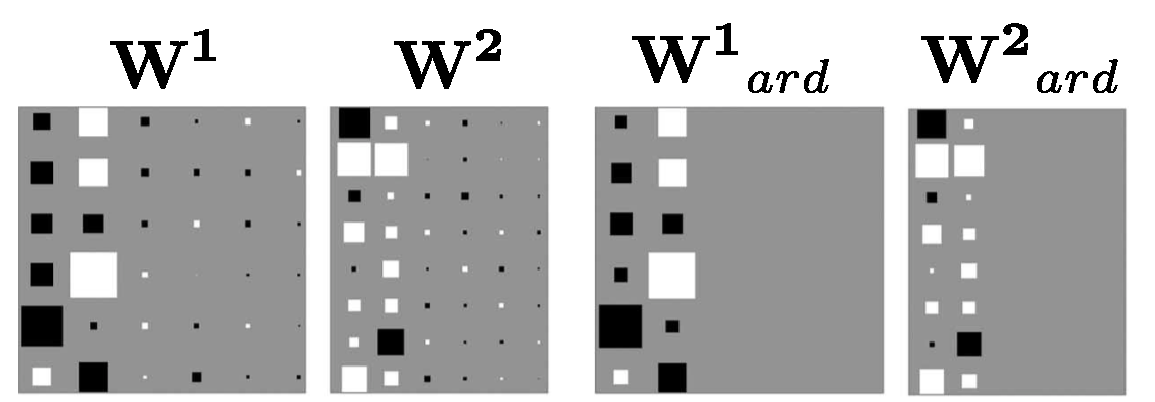
\includegraphics[width=0.85\linewidth]{hinton_cca}
	\caption{Comparison of the Hinton's diagram of $\bfW^{1}$ and $\bfW^{2}$ for the maximum likelihood CCA model (two left plots) and the variational bayes CCA model (two right plots). Reprinted from \cite{Wang2007} with modifications.}
	\label{fig:hinton_cca}
\end{figure}


\subsubsection{Group Factor Analysis} \label{section:gfa}

Group Factor Analysis (GFA) is the natural generalisation of Bayesian Canonical Correlation Analysis to an arbitrary number of views.
The original idea was originally presented in \cite{Virtanen2012} and a series of generalisations followed, tailored with specific assumptions for different applications \cite{Klami2015,Leppaaho2017,Bunte2016,Khan2014,Zhao2016,Remes2015}. In this section we will outline the core principle of GFA.

Given a data set of $M$ views $\bfY_1, \cdots, \bfY_M$, the task of GFA is to find $K$ factors that capture the variability \textit{within} as well as the variability \textit{between} views. In other words, we want to capture factors that not only explain variance that is shared across all views but we also want to capture factors that explain variance within a single view or between different subsets of views.\\
The starting point is to generalise the Bayesian CCA model (\Cref{section:bayesian_cca}) to $M$ views:
\begin{align*}
	\bfY^{1} &= \bfW^{2} \bfZ + \epsilon^{1} \\
	\bfY^{2} &= \bfW^{2} \bfZ + \epsilon^{2} \\
	& \cdots \\
	\bfY^{M} &= \bfW^{M} \bfZ + \epsilon^{M}
\end{align*}
Notice that there is a common factor space for all views, but there is a view-specific weight matrix. The key to disentangle the activity of each factor in each view lies on the sparsity structure imposed in the weights. Intuitively, if a facto $k$ is not driving any variation in a specific view $m$ we want all the individual weights to be pushed to zero. As shown before, this behaviour can be achieved using Automatic Relevance Determination (ARD) priors. However, if we were to use the same approach as in Bayesian CCA, where the ARD prior for factor $k$ is shared across all views, then factors would be restricted to have the same activity across all views.\\
In GFA this is generalised as follows:
\begin{align}
	p(\bfW) &= \prod_{m=1}^{M} \prod_{k=1}^{K} \Ndist{\bfw_{:,k}^m}{0,\frac{1}{\alpha_k^m}} \\
	p(\balpha) &= \prod_{m=1}^{M} \prod_{k=1}^{K} \Gdist{\alpha_k^m}{a_0^\alpha, b_0^\alpha}
\end{align}
This is effectively setting an ARD prior per factor $k$ and view $m$. The matrix $\balpha \in \R^{M \times K}$ defines four types of factors: (1) Inactive factors that do not explain variance in any view, which corresponds to all values $\balpha_k$ being large. (2) Fully shared factors that explain variance across all views, which corresponds to all values $\balpha_k$ being small. (3) Unique factors that explain variance in a single view, which corresponds to all values $\balpha_k$ being large, except for one entry. (4) Partially shared factors that explain variance in a subsets views, which corresponds to a mixture of small and large values for $\balpha_k$.\\

The corresponding graphical model is:

\begin{figure}[H] \begin{center}
	% \begin{tikzpicture}

% % Define nodes
% \node[obs, xshift=-1.5cm] (Y1) {$y^{m}_{n,d}$};

% \node[latent, below=of Y1, yshift=+0.5cm, xshift=+1.5cm] (Z) {$z_{n,k}$};

% \node[latent, double, double distance=1pt, below=of Y1, xshift=-1cm, yshift=-1cm] (W1) {$w^{1}_{d,k}$};
% \node[latent, double, double distance=1pt, below=of Y2, xshift=+1cm, yshift=-1cm] (W2) {$w^{2}_{d,k}$};

% \node[latent, double, double distance=1pt, left=of Y1, yshift=-0.5cm] (Tau1) {$\tau^{1}$};
% \node[latent, double, double distance=1pt, right=of Y2, yshift=-0.5cm] (Tau2) {$\tau^{2}$};

% % Connect the nodes
% \edge {Z} {Y1};
% \edge {Z} {Y2};
% \edge {W1} {Y1};
% \edge {W2} {Y2};
% \edge {Tau1} {Y1};
% \edge {Tau2} {Y2};
% % \edge {Z,W, Tau} {Y};

% % Plates
% \plate[] {plateK} {(Z)(W1)(W2)} {$K$};
% % \plate[] {plateN} {(Y1)(Y2)(Z)(plateD1.north)} {$N$};
% % \plate[] {plateD1} {(Y1)(W1)(plateK.south)(plateN.north)} {$D_1$};
% % \plate[] {plateD2} {(Y2)(W2)(plateK.south)(plateN.north)} {$D_2$};
% \plate[] {plateN} {(Y1)(Y2)(Z)} {$N$};
% \plate[] {plateD1} {(Y1)(W1)(Tau1)} {$D_1$};
% \plate[] {plateD2} {(Y2)(W2)(Tau2)} {$D_2$};

% \end{tikzpicture}



\begin{tikzpicture}
  % Define nodes:
  % matrix factorisation level
  \node[obs]   (Y) {$y_{n,d}^m$};
  \node[latent, above=of Y, xshift=-1.5cm] (Z) {$z_{n,k}$};
  \node[latent, above=of Y, xshift=1.5cm] (W) {$w^m_{k,d}$};
  % \node[latent, xshift=1.5cm] (Tau) {$\tau^m_{d}$};
  \node[latent, xshift=2.5cm] (Tau) {$\tau^m$};
  \node[latent, above=of W] (alpha) {$\alpha^m_{k}$};

  % Connect the nodes
  \edge {Z,W,Tau} {Y}; %
  \edge {alpha} {W};

  % Plates
  \plate[] {plateK} {(Z)(W)(alpha)} {$K$};
  \plate[] {plateN} {(Y)(Z) (plateK.south west)} {$N$};
  % \plate[] {plateD} {(Y)(W) (plateK.south east) (plateN.south east) (plateN.north east)} {$D_m$};
  \plate[] {plateD} {(Y)(W)} {$D_m$};
  % \plate[] {plateM} {(Tau) (plateK.north east)(plateD.south east)(plateD.south west)} {$M$};
  \plate[] {plateM} {(Y)(W)(Tau)(alpha)} {$M$};
\end{tikzpicture}

	\label{fig:graphical_GFA}
	\caption{Graphical model for Bayesian Group Factor Analysis}
\end{center} \end{figure}


% The following figure illustrates a representative GFA solution for three views:
% \begin{figure}[h]
% 	\centering
% 	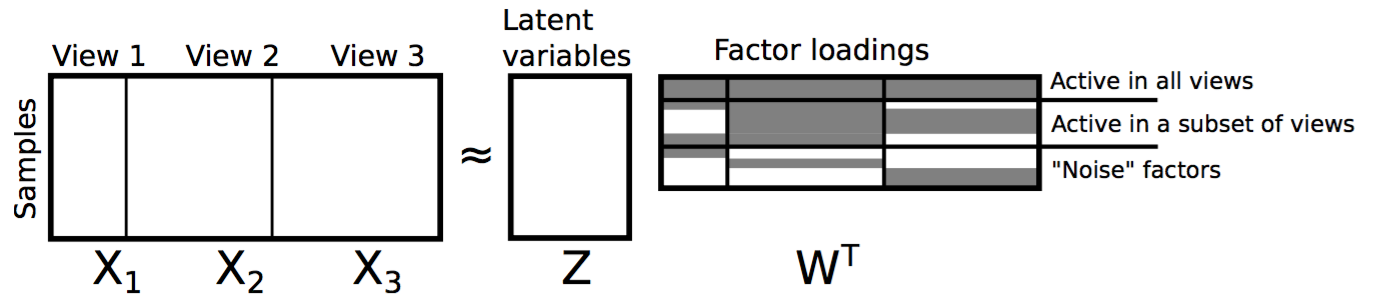
\includegraphics[width=1.0\linewidth]{GFA}
% 	\caption{(RE-DO FIGURE) Illustration of the GFA solution for $M=3$. The data sets are concatenated into a single matrix $\bfY$, which is factorised into a product of the latent variable matrix $\bfZ$ and a concatenated loading matrix $\bfW$. The shade in $\bfW$ depicts the factor and view-wise sparsity, where gray shading indicates high activity (small $\alpha_m^k$ value) and no shading indicates low activity (large $\alpha_m^k$ value). Note that some factors are active across all views (top), some factors are active in subsets of views (middle) and some factors are active in a single view (bottom).}
% 	\label{fig:intro:gfa}
% \end{figure}

Finally, notice that if $M=1$ the model reduces to Bayesian PCA (\Cref{section:bayesian_pca}), but when $M=2$ the model does \textit{not} reduce to Bayesian CCA because in the GFA setting factors are also allowed to capture both inter-specific variability (i.e. across views) intra-specific variability (within a view). In Bayesian CCA, the views share a common ARD prior per factor to enforce the factors to explain variation in both views, at the expense of ignoring sources of variability that are specific to a single view.

% \subsubsection{Similar approaches}
% Y. Jia, M. Salzmann, and T. Darrell. Factorized la- tent spaces with structured sparsity. In Advances in Neural Information Processing Systems 23, pages 982-990, 2010.

% GFA extends multi-battery factor analysis (MBFA), introduced by McDonald [4] and Browne [5] as a generalization of inter-battery fac- tor analysis (IBFA)

% Archambeau et al. [19] and Deleus et al. [20] extend CCA for M > 2, but instead of GFA they solve the more limited problem of multiple-battery factor analysis

% The MBFA models provide one set of factors that describe the rela- tionships between all groups, and then model the varia- tion specific to each group either with a free covariance matrix or a separate set of factors for that group. Besides the multi-set extensions of CCA, also the probabilistic interpretation of sparse matrix factorization [21], and the JIVE model for integrated analysis of multiple data types [22], [23] belong to the family of MBFA models

% \subsubsection{Extensions}
% Multiple extensions from the initial GFA framework have been proposed:

% \begin{itemize}
% 	\item Klami et al, 2015 \cite{Klami2015}: in the GFA framework outlined above, $\balpha \in \R^{M,K}$ is drawn from a flat gamma prior where views and factors are assumed independent. To encourage the model to find correlations between views, they specify a low-rank decomposition for $\balpha$:
% 	\[
% 		\log \balpha = \bfU \bfV^T + \bmu_{u}^T + \bmu_{v}^t
% 	\]
% 	with corresponding priors for $\bfU$ and $\bfV$. This representation directly captures correlations between the view activation profiles and is particularly useful when dealing with large number of views \cite{Klami2015}.

% 	\item Zhao et al, 2016 \cite{Zhao2016}: in the GFA framework outlined above, $\bfW^M$ have no element-wise sparsity. In this study, they implemented a more sophisticated structured sparsity prior called the three parameter beta prior \cite{Armagan2011}. The advantage of this prior distribution is three-fold: (1) it regularises the matrix, globally, removing factors that do not explain variation in any view. (2) Shrinks columns $\bfw_{:,k}^{m}$ to obtain the desired factor and group-wise sparsity. (3) Introduces feature-wise sparsity for each element $w_{d,k}^{m}$
 
% 	% \item Remes et al, 2015 \cite{Remes2015}: 

% 	% \item Bunte et al, 2016 \cite{Bunte2016}:

% 	% 	Biclustering is tradition- ally defined as simultaneously clustering both rows and columns in a data matrix
% 	% his is done simi- larly to how Khan et al. (2014) produced variable-wise sparsity, but now for both variables and samples to produce biclusters. Namely we use the following spike and slab priors (Suvitaival et al. (2014) included sparsity for samples 

% 	% 	We present a Bayesian approach for joint biclustering of multiple data sources


% \end{itemize}

